\chapter{经典方案介绍}
\vspace{-0.2cm}
本节将介绍涉及到的一些基础知识,包括$k-$近邻问题、密码学基础、语义安全、同态加密、Paiiler公钥加密。
\section{K近邻问题}
K近邻算法(K-Nearest Neighbor algorithm),简称KNN算法,属于分类算法,也是数据挖掘算法常用算法之一。K近邻算法即给定一个训练数据集,一个新的输入实例,在训练数据集中找出与该输入实例最邻近的K个实例,若这K个实例中多数属于某个类别,则该实例就属于这个类。
\begin{figure}[H]
\centering
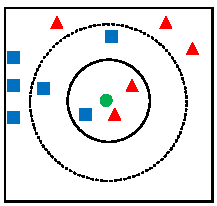
\includegraphics[width=6cm]{fig/KNN.pdf}
\caption{K近邻示意图} %\vspace*{-1.0cm}
\label{fig:KNN_pdf}
\end{figure}
如上图\ref{fig:KNN_pdf}所示,图中有两种不同的样本数据,分别用蓝色的正方形和红色的三角形表示,途中绿色的圆圈表示待分类的实例。现在假设我们并不知道途中绿色圆圈属于哪一个类别(即不知道属于蓝色小正方形还是红色三角形)。接下来依次取不同的K值,观察绿色圆圈所属的类别。
\begin{itemize}
\item $K=3$,则距离绿色圆圈最近的3个邻居分别为2个红色三角形和1个蓝色正方形,因此根据统计学的方法,基本可以判定绿色小圆圈属于红色三角形的类别。
\item $K=5$,观察可以发现,距离绿色圆点最近的5个邻居分别是2个红色三角形和3个蓝色正方形,基于统计方法,基本可以判定绿色小圆圈属于蓝色正方形。
\end{itemize}
通过上述观察我们可以发现,当无法判定当前待分类点从属于已知类别中的哪一类的时候,可以根据统计学方法观察待分类点所处位置的特征,衡量它周围邻居的权重,从而将待分类点归为权重更大的那一类。

KNN的算法描述大体可以分为以下三步骤:
\begin{itemize}
\item 依公式计算 待分类点Item 与 已知分类点$D_1$,$D_2$,...,$D_j$ 之相似度。得到Sim(Item, D1)、Sim(Item, D2)… …、Sim(Item, Dj)。
\item 对Sim(Item, $D_1$)、Sim(Item, $D_2$)… …、Sim(Item, $D_j$排序,若超过相似度阈值t则放入邻居案例集合NN。
\item 取出邻居案例集合NN中的前k个,求出这K个所属的类别,依多数决,得到Item 可能类别。
\end{itemize}

\section{密码学基础}
密码体制分为对称密码体制和非对称密码体制。对称密码体制也称为私钥密码体制,其加密方和解密方使用同一把密钥,一个私钥密码体制一般由三部分组成,一个密钥生成算法$G$(),一个加密算法$E$(),一个解密算法$D$()组成,可以表示为($G$,$E$,$D$),常用的对称加密算法有DES,AES等。非对称密码体制又叫做公钥密码体制,加密方和解密方采用不同的密钥,用来加密的密钥称为公钥,用来解密的密钥称为私钥。常用的公钥加密算法有RSA,ElGamal等。
\subsection{参与者与攻击者}
\paragraph{参与者}
参与者的行为通常决定了计算协议设计的难易程度,根据参与者在协议中的行为,可以将参与者分为三种类型。

\subparagraph{诚实的参与者}诚实参与者是指在协议过程中参与者完全按照协议的要求完成各个步骤,并且对自己的输入以及中间结果进行保密。诚实参与者可以根据自己的输入以及输出信息推导出其他参与者的信息。

\subparagraph{半可信的参与者}半可信的参与者是指在协议过程中,参与者完全按照协议的要求完成协议的各个步骤,并且可以将自己的输入以及输出信息透露给攻击者。诚实的参与者与半可信参与者的唯一区别就在于半可信的参与者可能会被攻击者妥协。

\subparagraph{恶意的参与者}恶意的参与者是指在协议过程中,参与者完全按照协议的要求完成协议的各个步骤,但参与者不会将自己的输入以及输出信息透露给参与者,并且可以根据攻击者的意图对输入以及输出信息进行改变,甚至对协议进行终止。
\paragraph{攻击者}
外部攻击者对恶意参与者的控制程度大致可以分为以下几种情形:

\subparagraph{被动攻击者}被动攻击者有可以称为监听者,他不会去控制恶意参与者的行为,其主要职责就是负责监听恶意参与者的输入、输出以及一些中间结果,

\subparagraph{主动攻击者}此类攻击者除了会对恶意参与者的输入、输出以及中间结果进行监听外还会对恶意参与者的行为进行控制。

\subsection{攻击类型}
根据密码分析者破译时已具备的前提条件,人们通常将攻击类型分为五种:唯密文攻击(ciphertext—only attack)、已知明文攻击(known plaintext attack)、选择明文攻击(chosen plaintext attack)、选择密文攻击(chosen ciphertext attack)、选择文本攻击(chosen text attack)。
\paragraph{唯密文攻击} 密码分析者除了拥有截获的密文外,没有任何其他可以利用的信息,分析者通过对这些截获的密文进行分析得出明文或密钥信息。
\paragraph{已知明文攻击} 密码分析者除了掌握相当数量的密文信息,还掌握了一些明文和用同一个密钥加密这些明文所对应的密文。
\paragraph{选择明文攻击} 密码分析者不仅可以获得一定数量的明-密文对,还可以选择任何明文并在使用同一未知密钥的情况下能到到相应的密文。
\paragraph{选择密文攻击} 密码分析者可以获得被加密密文所对应的明文,密码分析者的任务是推断出密钥以及其他密文信息所对应的明文。
\paragraph{选择文本攻击} 选择文本攻击是选择明文和选择密文攻击的结合。

\section{语义安全}
加密算法通常需要有三个必备的部分,分别是:原始消息$m$,加密密钥$k$以及加密算法。加密通常是为了对消息进行保密,最终目的就是为了在别人没有密钥的情况下,不能够从加密结果中恢复出原始的消息。

证明语义安全通常需要两种角色:攻击者(Adversary)和挑战者(Challenger)。 攻击者是指攻击加密算法的人,而挑战者是指接收攻击者挑战的人。Challenger持有密钥$k$,Adversary的目的就是观察Challenger运行加密算法后,输出的加密结果是否"看起来一样"。下面定义两个实验来具体讲解Adversary和Challenger:\\
实验0:
\begin{itemize}
    \item Adversary 任意选择两个消息$m_0,m_1$。
    \item Adversary将两个消息$m_0,m_1$发送给Challenger。
    \item Challenger运行加密算法,加密消息$m_0$,并将加密结果发送给Adversary。
\end{itemize}
实验1:
\begin{itemize}
    \item Adversary 任意选择两个消息$m_0,m_1$。
    \item Adversary将两个消息$m_0,m_1$发送给Challenger。
    \item Challenger运行加密算法,加密消息$m_1$,并将加密结果发送给Adversary。
\end{itemize}
Adversary的目的就是通过观察加密结果,判断加密结果是属于$m_0$还是$m_1$的加密结果值。上述两个实验的唯一区别就在于挑战者返回的是$m_0$还是$m_1$的加密结果。上述两个实验可以合并为一个实验,即:\\
实验b:
\begin{itemize}
    \item Adversary 任意选择两个消息$m_0,m_1$。
    \item Adversary将两个消息$m_0,m_1$发送给Challenger。
    \item Challenger运行加密算法,加密消息$m_b$,并将加密结果发送给Adversary。
\end{itemize}
如果Challenger能够以1/2的概率执行实验0,以1/2的概率执行实验1。那么,如果Adversary只有1/2的概率判断正确的加密结果,即有:
\begin{center}
    $Pr[c \leftarrow E(k,m_0)]=\frac{1}{2}$\\
    $Pr[c \leftarrow E(k,m_1)]=\frac{1}{2}$
\end{center}
这时候引入Adversary成功的优势的概念,成功优势是指如果Challenger以1/2 的概率执行实验0,以1/2的概率执行实验1,那么Adversary是否能够有比1/2 更大的概率猜测正确。因为Adversary 能够利用的只有加密结果值。因此如果有更大的概率,那么概率的增加只能是从加密结果中得来的。我们定义:
\begin{center}
    $Adv_{ss}[A,E]=|P_r[c \leftarrow E(k,m_0)]-Pr[c \leftarrow E(k,m_1)]|$
\end{center}
若攻击者的一点优势也没有,那么这个优势则为0,根据上面的定义有:
\begin{center}
    $Adv_{ss}[A,E]=|P_r[c \leftarrow E(k,m_0)]-Pr[c \leftarrow E(k,m_1)]|=|\frac{1}{2}-\frac{1}{2}|=0$
\end{center}
若加密结果能够反映出任何有关加密结果的消息,那么Adversary 成功的几率就会增加,即Adversary能够以更大的概率判断加密结果属于$m_0$还是$m_1$,这个时候有:
\begin{center}
$Pr[c \leftarrow E(k,m_0)]=\frac{1}{2}\pm\frac{1}{2}\varepsilon,pr[c\leftarrow E(k,m_1)]=\frac{1}{2}\mp\frac{1}{2}\varepsilon$
\end{center}
其中$\varepsilon$属于Adversary增加的概率,这时候Adversary 的攻击优势为:
\begin{center}
$Adv_{ss}[A,E]=|Pr[c\leftarrow E(k,m_0)]-Pr[c \leftarrow E(k,m_1)]|=|\frac{1}{2}\pm \varepsilon - \frac{1}{2}\mp \varepsilon|=\varepsilon$
\end{center}
由于Adversary拿到了加密结果,因此成功的优势一定会有所增加。密码学中定义,这个优势在多项式复杂度内可忽略就可以了,即这个优势小到无法用一个以位数为基本单位ude多项式来描述。比如,对于一个128位安全常数的加密算法,安全常数通常可以达到$1/2^{128}$:位数是128位,那么成功的优势为$2^{-128}$,可以发现,这不是一个有关位数的多项式,而是一个指数式。

综上可以发现,语言安全性的定义是一种基于游戏的安全定义。
\section{同态加密}
同态加密(Homomorphic Encryption)最早由Ron Rivest,Leonard Adleman就以银行为背景提出的。Craig Gentry第一次构造出了全同态的加密方案。同态加密方案关注的是数据处理安全,它提供了一种对加密数据进行处理的功能,即别人可以对数据进行相应的处理,但处理过程成不会泄露任何关于原始内容的信息,同时拥有密钥的用户对处理后的数据进行解密,得到的结果与对明文进行相应处理的结果一样。例如,Alice想让金匠加工一把金锁,但是金匠有可能会偷取部分金子,因此Alice想出了一种方法能够避免工人偷取金子。
\begin{itemize}
\item Alice首先将金子锁在一个密封住的盒子里面,并且在盒子上安装了一个手套。
\item 工人加工金子的时候需要带上手套,但是盒子是锁住的,所以工人是拿不到金块,就算是金块叫加工掉下来的碎片也得不到。
\item 待工人加工完后,Alice将盒子收回来,并用钥匙将盒子打开,得到加工后的产品。
\end{itemize}
这里面的盒子对应着加密算法、盒子上面的锁对应着用户持有的密钥、将金块放入盒子并且锁上对应着用同态加密方案对数据进行加密、工人加工的过程即阐明了同态的特性,即在无法取得数据的条件下对加密数据进行相应的处理、最后的开锁对应着对处理后的加密数据进行解密,得到处理后的结果。

同态加密在云计算中有很好的应用场景,几乎就是为云量身打造的,我们可以考虑如下的应用场景:假如一个用户想要处理某个数据,但是由于自身计算机硬件设备较差,不能对数据进行处理。这时候他可以使用云计算的概念,通过云来进行相应的处理从而得到结果。但是用户如果将数据不做任何处理直接交给云的话,可能会造成隐私泄露以及其他的一些安全问题。这时候,用户可以通过同态加密,然后通过云来对加密数据进行直接处理,并将处理后的结果返回给用户。这样的话用户向云服务提供商付款得到了处理后的结果,云服务提供商在不知道用户原始数据的情况下处理数据。

云计算应用场景下同态加密处理数据的整个过程如下:
\begin{itemize}
    \item Alice加密数据,并将加密后的数据外包给云服务提供商。
    \item Alice向云提交数据的处理方法(函数),这里用$f$表示。
    \item 云服务提供商根据函数$f$对数据进行相应的处理,并且将处理后的结果发送给Alice。
    \item Alice 收到函数$f$处理后的数据后,使用自己的密钥对数据进行解密,得到结果。
\end{itemize}
我们可以很直观的得到同态加密方案应该包含的一些函数:
\begin{itemize}
    \item 密钥生成函数(KeyGen): KeyGen函数由Alice 运行,产生用于加密原始数据(Data)的密钥(key),这期间可能会包含一些公开常数(PP)。
    \item 加密函数(Encrypt): Encrypt由Alice运行,用生成的密钥Key对用户数据Data进行加密,得到密文(CT)。
    \item 评估函数(Evaluate): Evaluate函数由云服务提供商进行运行,根据用户给定的数据处理函数$f$,对密文进行相应的处理,得到结果相当于用密钥对$f$(Data)进行操作。
    \item 解密函数(Decrypt):Decrypt由Alice运行,用于得到云服务提供商处理后的结果$f$(Data)。
\end{itemize}
根据数据处理函数$f$,实际上同态加密方案可以分为两类:
\begin{itemize}
    \item 全同态加密方案(Fully Homomorphic Encryption,FHE):FHE意味着可以支持任意给定的处理函数$f$,只要函数$f$可以通过算法描述,能够计算机实现即可。虽然FHE方案是一个很好的方案,也非常强大,但由于计算开销很大,通常无法在实际生产中使用。
    \item 半同态加密方案(Somewhat Homomorphic Encryption,SWHE):SWHE意味着数据处理函数只支持一些特定的函数$f$。SWHE方案相对FHE来说比较弱,但开销也相应的会变小不少,容易实现,因此在实际的项目中可以实现。
\end{itemize}
同态加密方案的最基本安全性是语义安全性,即密文不会泄露任何关于明文的信息,语义安全的具体介绍可以见上一节的描述。

有时候可能需要保护数据机密的同时数据处理函数$f$也需要保密,直观的说就是,云服务提供商不仅得不到任何关于原始数据的信息,连数据是如何处理的也不知道,只能按照给定的算法执行,然后返回用户所需要的结果。这种特性很是厉害,不过现在还没有FHE,甚至连SWHE也没有。
\section{Paillier公钥加密}
设$n$=$pq$,其中$p$,$q$为大素数,$\varphi(n)$ =$(p-1)(q-1)$,$\varphi(n)$为欧拉函数。Caemichael函数$\lambda(n)$ =$lcm(p-1)(q-1)$($lcm$代表最小公倍数)。$|{Z_{n^2}}^*|$ =$\varphi({n}^2)$ = $n\varphi(n)$,$\forall \omega \in {Z_{n^2}}^*$,为了方便表示,接下来所有的$\lambda(n)$直接用$\lambda$ 进行表示。根据Caemichael的性质,有${\omega}^\lambda$=$1 mod n$,${\omega}^{n\lambda}$ =$1 mod {n}^2$。

Paillier公钥密码体制是基于困难问题假设的,设$n=pq$,其中$p,q$为大素数,$g \in {Z_{n^2}}^*$,整数值的函数$\varepsilon_g$定义如下:$Z_n\times {Z_n}^* \rightarrow {Z_{n^2}}^* $,$(x,y) \rightarrow {g}^x \cdot {y}^n mod {n}^2$。如果$g$在${Z_{n^2}}^*$中的阶为$n$的倍数,则$\varepsilon_g$是一一映射。这样的话对于给定的$\omega \in {Z_{n^2}}^*$,$x \in Z_n$,则$\exists y \in {Z_n}^*$,使得$\varepsilon_g(x,y) = \omega$。这样的$\varepsilon_g (x,y)$ 称为$\omega$ 的n-residuosity class,用$[[\omega]]_g$表示。目前认为,对于给定的$n,g,\omega$,计算$[[\omega]]_g$是困难问题,即所谓的Composite Residuosity Assumption(CRA)。 但是根据$p,q$的内容,即依据$\lambda$,可以计算出任意的$[[\omega]]_g$。事实上,设$S_n={u<{n}^2 | u =1 mod n}$,$\forall u \in S_n$,$L(u)= \frac{u-1}{n} $,则有如下的结果:$[[\omega]]_g= \frac{L({\omega}^\lambda mod {n}^2)}{L({g}^\lambda mod {n}^2)} mod n$。\\
Paillier的加解密过程分为三个部分:
\begin{itemize}
\item 初始化阶段:$n=pq$,其中$p,q$为大素数,选取$g \in {Z_{n^2}}^* $,使得$gcd(L({g}^\lambda mod {n}^2)\\,n)=1$,gcd代表最大公约数,其中公钥pk为$(n,g)$,私钥sk为$(p,q)$ 等价为$\lambda(\lambda=lcm(p-1,q-1))$。
\item 加密阶段:设有明文$m \in Z_n$,且$m<n$。选择一个随机数$r<n$,则密文为$c={g}^m\cdot {r}^n mod {n}^2$。
\item 解密阶段:密文$c<{n}^2$,明文$m=\frac{L({\omega}^\lambda mod {n}^2)}{L({g}^\lambda mod {n}^2)} mod n$。

\end{itemize}
Pailler公钥加密方案满足加法和乘法同态:
\begin{itemize}
\item 加法同态:$D_{sk}(E_{pk}(a+b)) = D_{sk}(E_{pk}(a)*E_{pk}(b)mod {N}^2)$。其中$E_{pk}$()表示使用公钥加密,$D_{sk}$表示使用私钥进行加密。
\item 乘法同态:$D_{sk}(E_{pk}(a*b)) = D_{sk}(E_{pk}(a)^b mod N^2)$。其中$E_{pk}$()表示使用公钥加密,$D_{sk}$表示使用私钥进行加密。
\end{itemize}
\section{本章小结}
本章主要对隐私保护总的基础知识进行描述,包括$k-$近邻问题、密码学基础知识、语义安全、同态加密以及Pailler 公钥加密。

$k-$近邻问题介绍了基本概念,$k-$近邻算法属于分类算法,是数据挖掘中算法中常用算法之一。介绍中,通过案列对$k-$ 近邻问题进行了形象的描述,并在后续给出了$k-$ 近邻算法涉及到的三个重要步骤。

密码学基础中首先介绍了对称与非对称密码体制,对参与者与攻击者进行了介绍,其实中参与者含有诚实参与者、半可信参与者以及参与者,攻击者分为被动攻击者以及主动攻击者。攻击类型中,人们通常将其分为5种:唯密文攻击、已知明文攻击、选择明文攻击、选择密文攻击以及选择文本攻击。

语义安全部分以简单易懂的方式进行了讲解,语义安全实际上就是一种Adversary和Challenger之间进行的一种游戏。同态加密部分同意以案例的方式进行描述,同态加密在云计算中有很好的应用场景,几乎就是为云量身打造的,试想,如果有哪家存储公司能够将同态加密很好的应用起来,那么必将是一家独大,达到技术的垄断,可由于效率问题,目前为止还木有哪个全同态加密方案能够应用于实际的项目中。在Paillier中重点介绍了Paillier加解密过程中的三个步骤:初始化阶段,加密阶段以及解密阶段。Paillier公钥加密方案属于半同态加密方案,满足加法和乘法同态。
